\textbf{[TODO: find a consistent notation for Xnew, M, V and Madgraph model]}

\newcommand{\SUtwoUone}{\ensuremath{\mathrm{SU}(2)_{L} \times \mathrm{U}(1)_{Y}}\xspace}
\newcommand{\SUtwo}{\ensuremath{\mathrm{SU}(2)_{L}}\xspace}
\newcommand{\Lagr}{\ensuremath{\mathcal{L}}\xspace}
\newcommand{\fmet}{\ensuremath{f_{\mathrm{met}}}\xspace}
\newcommand{\met}{MET\xspace}
\newcommand{\ares}{\ensuremath{a_{\mathrm{res}}}\xspace}
\newcommand{\anonres}{\ensuremath{a_{\mathrm{non-res}}}\xspace}
\newcommand{\Xnew}{\ensuremath{X_{\mathrm{new}}}\xspace}
\newcommand{\BR}[2]{\ensuremath{\mathrm{BR}({#1} \to {#2})}\xspace}
\newcommand{\ssll}{\ensuremath{\ell^{+}\ell^{+}}\xspace}
\newcommand{\ttbarV}{\ensuremath{\ttbar V}\xspace}
\def\mfmet{\ensuremath{m(f_{\mathrm{met}})}}
\def\mvmet{\ensuremath{m(v_{\mathrm{met}})}}
\def\vmet{\ensuremath{v_{\mathrm{met}}}}
\def\fmet{\ensuremath{f_{\mathrm{met}}}}


A dark matter candidate $\chi$ and a new particle $M$ (vector or scalar) 
are added to the SM, in an effective theory that respects the $\SUtwoUone$ symmetry 
%%CD: effective theory???
and produces a single top quark in association with either the DM particle or the new particle
(generally called $\Xnew$ when no distinction is made). The full details of 
these models are described in~\cite{AndreaFuksMaltoni,Agram:2013wda,Boucheneb:2014wza}. 

There are two classes of models based on the monotop production mode: 
resonant and non-resonant production, as shown 
in Fig.~\ref{fig:feyn_prod}. 

The following two sections describe the phenomenology leading to these two production mechanisms.
Depending on the nature of $\Xnew$, two main final states might be relevant: 
monotop production or same-sign top quark pair production. 
The interplay of these two signatures can largely probe this class of dark matter model,
but a detailed study of their complementarity is beyond the scope of this Forum report. 

\begin{figure}[!h!tpd]
\centering
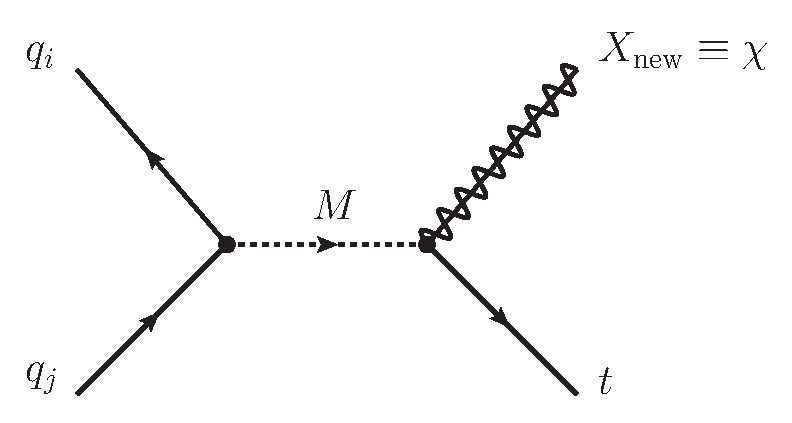
\includegraphics[width=0.31\textwidth]{figures/singletop/feyn_diags/Resonant}
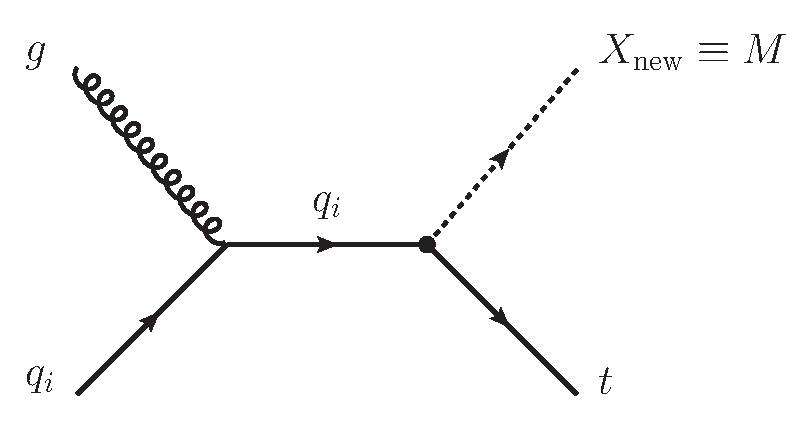
\includegraphics[width=0.31\textwidth]{figures/singletop/feyn_diags/NonResonant}
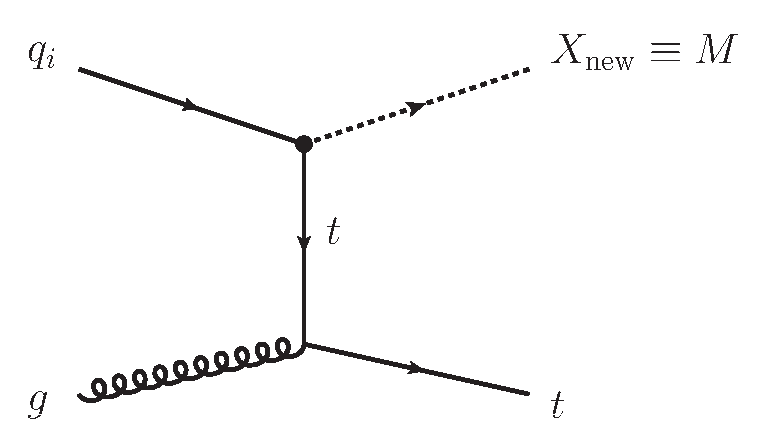
\includegraphics[width=0.31\textwidth]{figures/singletop/feyn_diags/NonResonant2}
%\subfigure[\label{subfig:S1}]{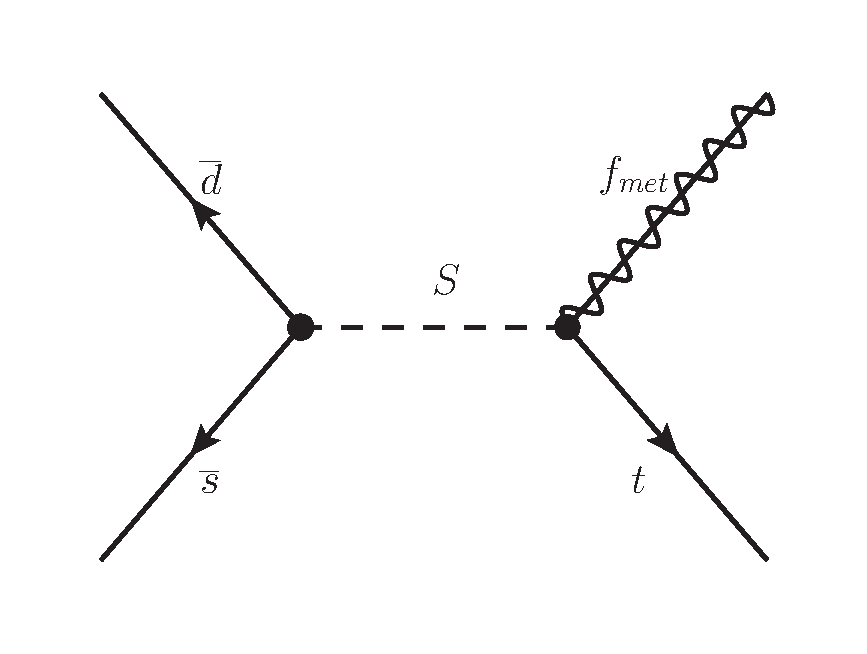
\includegraphics[width=0.46\textwidth]{feyn_diags/S1}}\\
%\subfigure[\label{subfig:S4_s}]{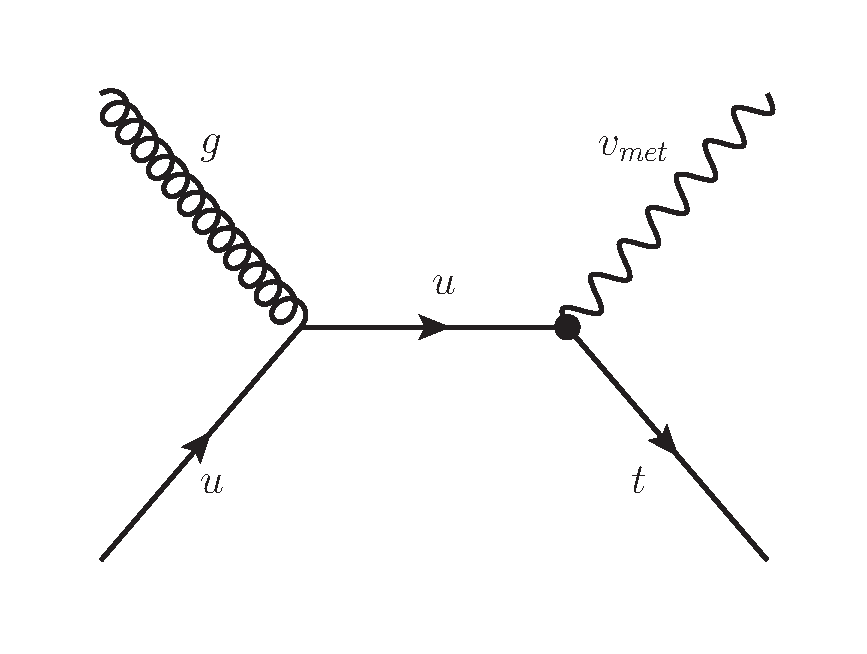
\includegraphics[width=0.46\textwidth]{feyn_diags/S4_s}}
%\subfigure[\label{subfig:S4_t}]{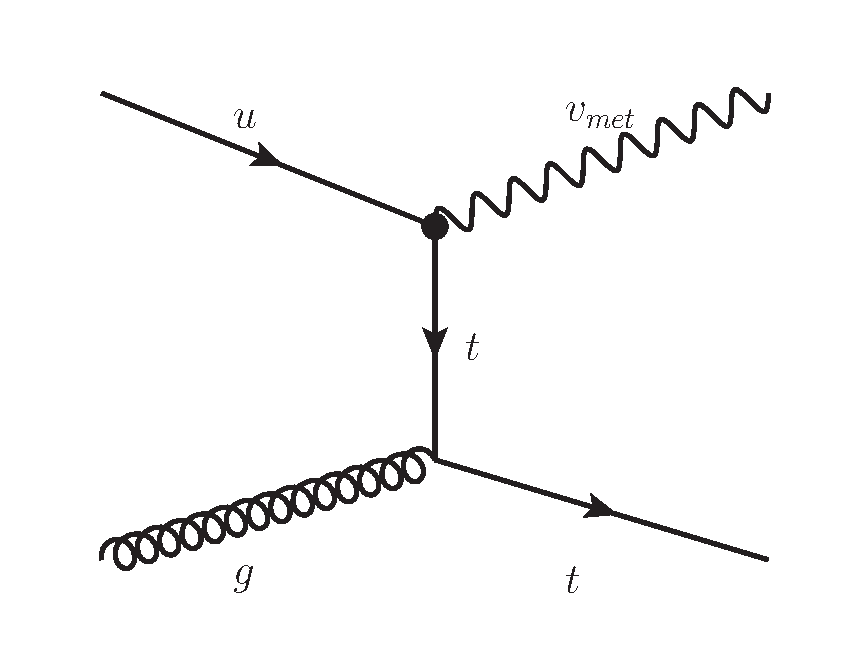
\includegraphics[width=0.46\textwidth]{feyn_diags/S4_t}}
\caption
{
%Feynman diagram of leading order processes leading to monotop events: production of
%a coloured scalar resonance $S$ decaying into a top quark and a spin-$1/2$ fermion $f_{met}$
%in the $\mathrm{S1_R}$ model~\subref{subfig:S1}, and $s$-\subref{subfig:S4_s}
%and $t$-\subref{subfig:S4_t} channel non resonant production of a top quark in association with
%a spin-1 boson $v_{met}$ in the $\mathrm{S4_R}$ model.
Feynman diagram of leading order processes leading to monotop events: resonant production of
$t$ via resonant new particle $M$ decaying into a top quark and $\Xnew$, which is the dark matter fermion $\chi$ (left),
and $s$ and $t$ channel non-resonant production of a top quark in association with $\Xnew$, which is the new particle $M$ (middle and right).
}
\label{fig:feyn_prod}

\end{figure}

\newthought{Resonant production}
\label{sec:ResonantProd}

In this case, the new particle $M$ is a couloured $2/3$-charged scalar $\phi^{\pm}$ decaying into a top quark and a spin-$1/2$ invisible particle, $\chi$ (in this case $\Xnew$ is the dark matter candidate $\chi$). 
The dynamics of the new sector is then described by the following Lagrangian:

\begin{eqnarray}
\label{eq:lagrangianResonant}
\mathcal{L} =  d^{C}_{i} \:  [ (g^{v}_{\phi d})^{ij} +  (g^{a}_{\phi d})^{ij} \gamma^{5} ] \: d_{j} \: \phi^{\pm}  +  u^{C}_{k}  [ (g^{v}_{u\chi})^{k} + (g^{a}_{u\chi})^{k} \gamma^{5} ] \: \chi \: \phi^{\pm}
%%CD: problems with the original typesetting
\end{eqnarray}
where $u$ ($d$) stands for any $up$-quark ($down$-quark), 
the index $v$ ($a$) stands for vectorial (axial), $C$ means charge conjugate and $i,j,k$ 
run over the generations (color indices involved in the $\phi^{\pm}-$quarks interaction are not explicitly written).
The first term leads to the production of the new particle and the last term allows its decay into a $up$-quark 
and a non interacting fermion (in particular to the top quark when $(g^{v/a}_{u\chi})^{k}$ 
is sizable mainly for $k=3$).
This model is then described by the masses of the new particle $m_{\phi}$ and the invisible 
fermion $m_{\chi}$, and the coupling 
$(g^{v/a}_{\phi d})^{ij}$ and $(g^{v/a}_{u\chi})^{k}$.
% 
% \com{Question/comment: in this resonant model, this is not so obvious to interpret $\phi_{\pm}$ as the new particle since there is a vertex $\phi-u-\chi$.
% It is somehow breaking the concept of having a dark sector weakly coupled to ordinary matter via a new particle.}
% 
% 
\newthought{Non-Resonant production}
\label{sec:NonResonantProd}

For the non-resonant production, the top quark is produced in association with the new particle 
($\Xnew$ is then the new particle and not the dark matter candidate). 
The new particle can be either a new scalar, interacting with the SM and the DM candidate, 
or a new vector. For simplicity, we only consider the case of a vector new particle, as the scalar case
would involve a mixing with the SM Higgs boson and therefore a larger parameter space. 

%%CD: Full explanation is below
% First, the new particle can be a scalar field interacting with the SM field and the dark matter
% candidate as described in this lagrangian:
% \begin{equation}
%  \label{eq:lagrangianNonResonantScalar}
% \mathcal{L} =  u^{C}_{i} \:  [ (g^{v}_{\phi u})^{ij} +  (g^{a}_{\phi u})^{ij}  \gamma^{5} ] \: u_{j} \: \phi  
%  +  \chi^{C}  [ g^{v}_{\phi\chi} + g^{a}_{\phi\chi}  \gamma^{5} ] \chi \: \phi
% \end{equation}
% where $u$ stands for any $up$-quark, the index $v$ ($a$) stands for vectorial (axial), 
% $C$ means charge conjugate and $i,j,k$ run over the generations.
% The first term describes the interaction between the new particle and the $up$-quarks while the 
% second term leads to the decay of the new particle into invisible fermions. 
% In this model, there is necessarily a mixing between $\phi$ and  the Higgs boson field. 
% Additional parameters are then required to describe this new sector: in addition to 
% the new particle mass and couplings, the mixing matrix of the two scalar fields
% is needed in order to make predictions. For the sake of simplicity, 
% we do not consider this case were the parameters space would be too large.

The dynamics of a case with a vector new particle follows this Lagrangian:
\begin{equation}
 \label{eq:lagrangianNonResonantVector}
  \mathcal{L}  =  \bar{u}_{i} [ (g^{v}_{Vu})^{ij} \gamma^{\mu} + (g^{a}_{Vu})^{ij} \gamma^{5} ] u_{j} \: V_{\mu}  
  +  \bar{\chi} [ g^{v}_{Vu} \gamma^{\mu} + g^{a}_{V\chi} \gamma^{5} ]   \chi \: V_{\mu}
\end{equation}
where $u$ stands for any $up$-quark, the index $v$ ($a$) stands for vectorial (axial) and $i,j,k$ run over the generations.
The first term describes the interaction between the new particle and the $up$-quarks while the second term leads to the decay the new particle 
into invisible fermions. The new sector can be defined with the couplings $(g^{v/a}_{Vu})^{ij}$, 
$g^{a/v}_{V\chi}$ and the masses $m_V$ and $m_{\chi}$. 
This model can be probed by two different experimental signatures: monotop and same-sign top quark production. 
% 
% \com{Question for theorists: why it cannot mix with $\Zboson$ in case of vectorial new particle ?}

\newthought{Model parameters and assumptions}
 
The models considered as benchmarks for the first LHC searches
contain further assumptions in terms of the flavour and chiral structure of the model
with respect to the full Lagrangians from  equations~\eqref{eq:lagrangianResonant} and~\eqref{eq:lagrangianNonResonantVector}.
These assumptions lead to limitations in LHC constraints of 
the parameter space of these models, qualitatively discussed below. 

\paragraph{Assumptions in the flavour structure of the models}

In order to be visible at the LHC in the monotop final state, 
these models must include a strong coupling between the new particle $\phi$ and $t\chi$.
In the resonant case, the new particle must also couple to light quarks in order
to be produced at the LHC, leading to possible constraints from
dijet searches. 
The same kind of assumption exists for the non-resonant production. 
The new particle $M$ must be produced from a light quark in the initial state, 
in association with a top quark: this signature can mainly probe a high 
coupling $\left(g^{v/a}_{Vu}\right)^{13}_{Vu} \equiv g^{v/a}_{Vtu}$. Therefore,
the sensitivity to other flavour couplings is significantly lower, since $V$ would be 
produced at a lower rate. 

%CD: not sure I understand?
% In addition, the new particle must decay into invisible particles
% to lead to the searched monotop final state. As a consequence, the sensitivity for 
% scenario where $\BR{V}{\chi\chi}\ll 100\%$ can be quite low. 
% To cope with this second limitation, a same-sign top quark final state 
% $gu \to tV(\to t\bar{u})$ is proposed to cover the cases where $V$ would decay
% into visible particles. This case is more likely as the $tV$ production rate increases, 
% and becomes then a key point to constraint this model in a consistent way.

% % \com{Questions for theorists:
% % \begin{itemize}
% %  \item How well these flavour assumptions are allowed by the other HEP data (proton decay life time, flavour physics, etc ...) ?
% %  \item MFV criteria ?
% % \end{itemize}
% % }
% 
% \subsubsection{Chiral structure}
% \label{sec:chiralstructure}
\paragraph{Assumptions in the chiral structure of the models}

We only consider right-handed quark components, in order to simplify the phenomenology. 
The representation of the left-handed components under the $\SUtwo$ symmetry would a 
coupling to $down$-type quarks, since the effective theory is invariant under $\SUtwoUone$ 
gauge symmetry. Having a coupling between the new particle and $down$-type quarks 
complicates the collider phenomenology in terms of decay modes. Typically, including 
the left-handed components of quarks in the lagrangian~\eqref{eq:lagrangianNonResonantVector} 
describing the $Vtu$ vertex would lead to 
\begin{equation}
 \mathcal{L}_{Vtu} \; = \;  g^{R}_{Vtu} \: \bar{t}_{R}\gamma^{\mu}u_R \: V_{\mu} \; + \; g^{L}_{Vtu} 
 (\bar{t}_{L}\gamma^{\mu}u_L \: + \:  \bar{b}_{L}\gamma^{\mu}d_L ) \: V_{\mu}
\end{equation}
where $g^{R/L} \equiv 1/2 \, (g^{v} \pm g^{a})$ couples only to right-handed/left-handed components. 
The second term stems from invariance under $\SUtwo$ rotations, and leads to an additional 
decay mode $V \to b\bar{d} + \bar{b}d$ (on top of $V \to t\bar{u} + \bar{t}u$ and $V \to \chi\chi$). 
\textbf{[Open point: do we just set the 2nd term to zero in this model? Justification?]}

\newthought{Implementation and notation}


This Section describes the notations used in the MadGraph model~\cite{MGmodel} convention, 
in term of the ones introduced in the previous Section.

The Madgraph model corresponds to the Lagrangian from~\cite{AndreaFuksMaltoni}. 
Each coupling constant of this dynamics can be set via the paramater card and 
the blocks which are relevant for the two models used for the experimental searches are described below.

\begin{enumerate}

\item Resonant scalar model described by the Lagrangian~\eqref{eq:lagrangianResonant}
  \begin{itemize}
  \item \texttt{AQS} and \texttt{BQS}: $3\times 3$ matrices (flavour space) fixing the coupling of the scalar $\phi^{\pm}$ ($S$ stands for scalar) and $down$-type 
    quarks ($Q$ stands for quarks), written in this note $g_{\phi u}$ or $a^{q}_{\mathrm{res}}$.
  \item \texttt{A12S} and \texttt{B12S}: $3\times 1$ matrices (flavour space) fixing the coupling of the fermion $\chi$ ($12$ stands for spin-$1/2$ fermion) 
    and $up$-type quarks, written in this note $g_{u \chi}$ or $a^{1/2}_{\mathrm{res}}$.
  \item particle name: the scalar $\phi^{\pm}$ is labelled $S$ and the fermion $\chi$ is $f_{met}$
  \end{itemize}  
  
\item Non-resonant vectorial model described by the Lagrangian~\eqref{eq:lagrangianNonResonantVector}
\begin{itemize}
\item \texttt{A1FC} and \texttt{B1FC}: $3\times 3$ matrices (flavour space) fixing the coupling of the vector $V$ 
  ($1$ stands for vector) and $up$-type quarks, written in this note $g_{Vu}$ or $a_{\mathrm{non-res}}$.
\item particle name: the vector $V$ is labelled $v_{met}$ and the fermion $\chi$ doesn't exist
\item the dark matter candidate $\chi$ is not implemented (this model assumes $\BR{V}{\chi\chi}=100\%$)
\end{itemize}

\end{enumerate}
% 
$A$ means vectorial coupling ($g^{v}$) and $B$ means axial coupling ($g^{a}$) and these two matrices 
are taken to be equal according to the chiral assumptions made above. 
The convention adopted follows \cite{ATLASmonotop} in defining 
a single number $a_{\mathrm{res}}$ ($a_{\mathrm{non-res}}$) 
for the resonant (non resonant) model, such as $(\ares^q)_{\mathrm{12}}=(\ares^q)_{\mathrm{21}}=(\ares^{1/2})_{\mathrm{3}}\equiv \ares$ 
(in order to have $d-s-S$ couplings, and $t-S-f_{met}$ couplings) 
and $(\anonres)_{\mathrm{13}}=(\anonres)_{\mathrm{31}}\equiv \anonres$ (in order to have $v_{met}-t-u$ couplings). 

\newthought{Parameter scan}

\textbf{[Open point - parameter scan studies go here.]}

 Which parameters impact the kinematics (this is the only relevant aspect form the experimental point of view)? 
 Some studies would be nice to put in this documents about:
 \begin{itemize}
  \item mediator mass
  \item mediator width: no effect (or parametrizable effects, plots are ready and need to be included)
  \item \textbf{which parameters} impact our experimental sensitivity? Which plane should be scanned?
 \end{itemize}

 What are the relevant numerical range to explore? First guess would be to follow the mono-top analysis.

\newthought{Parameter choices and cross sections}

\textbf{[Open point: update with new numbers]}

ATLAS has considered two models, a resonant and a non-resonant production, using only right-handed top quarks in the lepton+jets final state. The signal samples were produced with {\sc Madgraph5} v1.5.11 interfaced with {\sc Pythia} 8.175, using the MSTW2008LO Parton Distribution Function (PDF) set (lhapdf ID: 21000).
The mass of the top quark was set at 172.5 GeV. Dynamic renormalisation and factorisation scales were used.
The $\met$ particle mass was varied, and in the case of the resonant model the resonance mass was fixed at 500~GeV:
\begin{itemize}
\item Resonant model,  $\met$ particle mass: [0,100]~GeV in 20~GeV steps
\item Non-resonant model, $\met$ particle mass: [0,150]~GeV in 25~GeV steps, [200,300]~GeV in 50~GeV and [400,1000]~GeV in 100~GeV steps 
\end{itemize}

%\com{How to translate the monotop paper couplings to the notation of this note? }
The couplings $\ares$ and $\anonres$ are set at a fixed value of $0.2$.
In addition, two samples are produced for the resonant model for $\mfmet=100$~GeV,
with coupling strengths fixed at $\ares=0.5$ and $\ares=1.0$,
in order to check the effect of the resonance width on the signal event kinematics. 
The total width of the resonance varies quadratically with the coupling strength,
corresponding to a width of 3.5~GeV, 21.6~GeV, and 86.5~GeV at $\ares=0.2$, $\ares=0.5$, and $\ares=1.0$, respectively.

The number of free parameters is reduced by assuming $(\ares^q)_{\mathrm{12}}=(\ares^q)_{\mathrm{21}}=(\ares^{1/2})_{\mathrm{3}}\equiv \ares$
for the resonant model and $(\anonres)_{\mathrm{13}}=(\anonres)_{\mathrm{31}}\equiv \anonres$ for the non-resonant model,
all other elements of these coupling matrices being equal to 0.
For each model, the coupling parameter $\ares$ or $\anonres$ and the masses of the exotic particles are independent.

The cross-sections as well as the width of the resonance for the resonance model are shown in Table~\ref{tab:S1R_Xsec}.  
The cross-section is slowly decreasing when $m(f_{met})$ increases,
and the values do not differ by larger than 10\%, due to the similarity of the kinematics, in the chosen mass range.
\begin{table}[!htb]\centering
\begin{tabular}{l|r|r|r}
\hline \hline
% $\mathrm{m}(f_{\mathrm{met}})$ [GeV] & $\sigma\times\mathrm{BR(S\rightarrow t f_{met})}\times\mathrm{BR(t\rightarrow l^+\nu b)[pb]}$ & $\sigma\times\mathrm{BR(S\rightarrow t f_{met})}\times\mathrm{BR(t\rightarrow jjj)[pb]}$ & $\Gamma(S)$ [GeV]   \\
$m(f_{met})$ [GeV] & $\sigma_{lep}$~[pb] & $\sigma_{had}$~[pb] & $\Gamma(\Phi)$ [GeV]   \\
\hline \hline
0                        &  1.107              & 2.214               &  3.492  \\
20                       &  1.102              & 2.205               &  3.491  \\
40                       &  1.089              & 2.180               &  3.487  \\
60                       &  1.068              & 2.137               &  3.481 \\	
80                       &  1.039              & 2.078               &  3.472  \\
100                      &  1.001              & 2.003               &  3.461  \\
100 ($\ares=0.5$) &  6.091              &  12.13              & 21.63    \\
100 ($\ares=1.0$  &  21.77              &  43.72              &  86.52   \\
\hline \hline
\end{tabular}
\caption
{
Theoretical predictions for the product of the production cross-section of the
scalar resonance, the branching ratio of its decay into a top quark and the invisible particle,
and of the branching ratio of the top quark decay into a semi-leptonic ($\sigma_{lep}$) or fully-hadronic ($\sigma_{had}$) final state,
in the resonance model.
Values are given for a resonance of mass 500~GeV and for an effective coupling $\ares=0.2$ (except for two masses),
as a function of the mass $m(f_{met})$ of the neutral fermion.
The total widths $\Gamma(\Phi)$ of the resonance are also shown.
}
\label{tab:S1R_Xsec}
\end{table}


For the non-resonant case, the cross-sections are given in Table~\ref{tab:S4R_Xsec} and are calculated with $\anonres=0.2$.
The cross-section diverges when $m(v_{met})$ tends to 0~GeV.  However, when the mass is exactly 0~GeV the cross-section has a finite value,
due to the specificity of the propagator for this massless spin-1 boson.
\begin{table}[!htb]\centering
\begin{tabular}{l|r|r}
\hline \hline
% $m(v_{met})$ [GeV] & $\sigma\times\mathrm{BR(t\rightarrow l^+\nu b)[pb]}$ & $\sigma\times\mathrm{BR(t\rightarrow jjj)[pb]}$ \\
$m(v_{met})$ [GeV] & $\sigma_{lep}$~[pb] & $\sigma_{had}$~[pb] \\
\hline \hline
0                  &  96.03              & 192.4    \\
25                 &  359.0              & 717.9    \\
50                 &  113.4              & 226.9    \\
75                 &  59.86              & 119.5    \\
100                &  37.45              & 74.82    \\
125                &  25.35              & 50.68    \\
150                &  18.00              & 35.96    \\
200                &  9.662              & 19.28    \\
250                &  5.506              & 11.02    \\
300                &  3.328              & 6.656    \\
400                &  1.372              & 2.738    \\
500                &  0.6345             & 1.270    \\
600                &  0.3192             & 0.6354   \\
700                &  0.1698             & 0.3383   \\
800                &  0.09417            & 0.1883   \\
900                &  0.05472            & 0.1091   \\
1000               &  0.03259            & 0.06479  \\
\hline \hline
\end{tabular}
\caption
{
Theoretical predictions for the product of the production cross-section of the invisible vector $v_{met}$ and of a top quark,
and of the branching ratio of the top quark decay into a semi-leptonic ($\sigma_{lep}$) or fully-hadronic ($\sigma_{had}$) final state, 
in the non-resonance model.
Values are given for an effective coupling $\anonres=0.2$, as a function of the mass $m(v_{met})$ of the invisible state.
}
\label{tab:S4R_Xsec}
\end{table}

% \com{I think it might make more sense to have the joboption information in a public web site instead of
% adding all the details into the note. Reference only visible for ATLAS members: \\
% {\small https://svnweb.cern.ch/trac/atlasoff/browser/Generators/MC12JobOptions/trunk/gencontrol/MadGraphControl$\_$Monotop.py}}

\textbf{[Open point: systematic uncertainties]}
% \com{Question for DM forum:
% \begin{itemize}
%  \item Do we want to give more details about the Madgraph implementation, the couplings value in the param\_card, etc ... ?
%  \item I am not aware of any work on systematic variation due to scale, PDF choice, showering (Maybe some was done in the monotop analysis?). Then I am not completely what to put here.
% \end{itemize}
% }


